% Options for packages loaded elsewhere
% Options for packages loaded elsewhere
\PassOptionsToPackage{unicode}{hyperref}
\PassOptionsToPackage{hyphens}{url}
\PassOptionsToPackage{dvipsnames,svgnames,x11names}{xcolor}
%
\documentclass[
  norsk,
  a4paper,
]{article}
\usepackage{xcolor}
\usepackage{amsmath,amssymb}
\setcounter{secnumdepth}{3}
\usepackage{iftex}
\ifPDFTeX
  \usepackage[T1]{fontenc}
  \usepackage[utf8]{inputenc}
  \usepackage{textcomp} % provide euro and other symbols
\else % if luatex or xetex
  \usepackage{unicode-math} % this also loads fontspec
  \defaultfontfeatures{Scale=MatchLowercase}
  \defaultfontfeatures[\rmfamily]{Ligatures=TeX,Scale=1}
\fi
\usepackage{lmodern}
\ifPDFTeX\else
  % xetex/luatex font selection
\fi
% Use upquote if available, for straight quotes in verbatim environments
\IfFileExists{upquote.sty}{\usepackage{upquote}}{}
\IfFileExists{microtype.sty}{% use microtype if available
  \usepackage[]{microtype}
  \UseMicrotypeSet[protrusion]{basicmath} % disable protrusion for tt fonts
}{}
\makeatletter
\@ifundefined{KOMAClassName}{% if non-KOMA class
  \IfFileExists{parskip.sty}{%
    \usepackage{parskip}
  }{% else
    \setlength{\parindent}{0pt}
    \setlength{\parskip}{6pt plus 2pt minus 1pt}}
}{% if KOMA class
  \KOMAoptions{parskip=half}}
\makeatother
% Make \paragraph and \subparagraph free-standing
\makeatletter
\ifx\paragraph\undefined\else
  \let\oldparagraph\paragraph
  \renewcommand{\paragraph}{
    \@ifstar
      \xxxParagraphStar
      \xxxParagraphNoStar
  }
  \newcommand{\xxxParagraphStar}[1]{\oldparagraph*{#1}\mbox{}}
  \newcommand{\xxxParagraphNoStar}[1]{\oldparagraph{#1}\mbox{}}
\fi
\ifx\subparagraph\undefined\else
  \let\oldsubparagraph\subparagraph
  \renewcommand{\subparagraph}{
    \@ifstar
      \xxxSubParagraphStar
      \xxxSubParagraphNoStar
  }
  \newcommand{\xxxSubParagraphStar}[1]{\oldsubparagraph*{#1}\mbox{}}
  \newcommand{\xxxSubParagraphNoStar}[1]{\oldsubparagraph{#1}\mbox{}}
\fi
\makeatother


\usepackage{longtable,booktabs,array}
\usepackage{calc} % for calculating minipage widths
% Correct order of tables after \paragraph or \subparagraph
\usepackage{etoolbox}
\makeatletter
\patchcmd\longtable{\par}{\if@noskipsec\mbox{}\fi\par}{}{}
\makeatother
% Allow footnotes in longtable head/foot
\IfFileExists{footnotehyper.sty}{\usepackage{footnotehyper}}{\usepackage{footnote}}
\makesavenoteenv{longtable}
\usepackage{graphicx}
\makeatletter
\newsavebox\pandoc@box
\newcommand*\pandocbounded[1]{% scales image to fit in text height/width
  \sbox\pandoc@box{#1}%
  \Gscale@div\@tempa{\textheight}{\dimexpr\ht\pandoc@box+\dp\pandoc@box\relax}%
  \Gscale@div\@tempb{\linewidth}{\wd\pandoc@box}%
  \ifdim\@tempb\p@<\@tempa\p@\let\@tempa\@tempb\fi% select the smaller of both
  \ifdim\@tempa\p@<\p@\scalebox{\@tempa}{\usebox\pandoc@box}%
  \else\usebox{\pandoc@box}%
  \fi%
}
% Set default figure placement to htbp
\def\fps@figure{htbp}
\makeatother


% definitions for citeproc citations
\NewDocumentCommand\citeproctext{}{}
\NewDocumentCommand\citeproc{mm}{%
  \begingroup\def\citeproctext{#2}\cite{#1}\endgroup}
\makeatletter
 % allow citations to break across lines
 \let\@cite@ofmt\@firstofone
 % avoid brackets around text for \cite:
 \def\@biblabel#1{}
 \def\@cite#1#2{{#1\if@tempswa , #2\fi}}
\makeatother
\newlength{\cslhangindent}
\setlength{\cslhangindent}{1.5em}
\newlength{\csllabelwidth}
\setlength{\csllabelwidth}{3em}
\newenvironment{CSLReferences}[2] % #1 hanging-indent, #2 entry-spacing
 {\begin{list}{}{%
  \setlength{\itemindent}{0pt}
  \setlength{\leftmargin}{0pt}
  \setlength{\parsep}{0pt}
  % turn on hanging indent if param 1 is 1
  \ifodd #1
   \setlength{\leftmargin}{\cslhangindent}
   \setlength{\itemindent}{-1\cslhangindent}
  \fi
  % set entry spacing
  \setlength{\itemsep}{#2\baselineskip}}}
 {\end{list}}
\usepackage{calc}
\newcommand{\CSLBlock}[1]{\hfill\break\parbox[t]{\linewidth}{\strut\ignorespaces#1\strut}}
\newcommand{\CSLLeftMargin}[1]{\parbox[t]{\csllabelwidth}{\strut#1\strut}}
\newcommand{\CSLRightInline}[1]{\parbox[t]{\linewidth - \csllabelwidth}{\strut#1\strut}}
\newcommand{\CSLIndent}[1]{\hspace{\cslhangindent}#1}

\ifLuaTeX
\usepackage[bidi=basic]{babel}
\else
\usepackage[bidi=default]{babel}
\fi
% get rid of language-specific shorthands (see #6817):
\let\LanguageShortHands\languageshorthands
\def\languageshorthands#1{}


\setlength{\emergencystretch}{3em} % prevent overfull lines

\providecommand{\tightlist}{%
  \setlength{\itemsep}{0pt}\setlength{\parskip}{0pt}}



 


\usepackage{float}
\usepackage{tabularray}
\usepackage[normalem]{ulem}
\usepackage{graphicx}
\usepackage{rotating}
\UseTblrLibrary{booktabs}
\UseTblrLibrary{siunitx}
\NewTableCommand{\tinytableDefineColor}[3]{\definecolor{#1}{#2}{#3}}
\newcommand{\tinytableTabularrayUnderline}[1]{\underline{#1}}
\newcommand{\tinytableTabularrayStrikeout}[1]{\sout{#1}}
\makeatletter
\@ifpackageloaded{caption}{}{\usepackage{caption}}
\AtBeginDocument{%
\ifdefined\contentsname
  \renewcommand*\contentsname{Table of contents}
\else
  \newcommand\contentsname{Table of contents}
\fi
\ifdefined\listfigurename
  \renewcommand*\listfigurename{Figurliste}
\else
  \newcommand\listfigurename{Figurliste}
\fi
\ifdefined\listtablename
  \renewcommand*\listtablename{Tabelliste}
\else
  \newcommand\listtablename{Tabelliste}
\fi
\ifdefined\figurename
  \renewcommand*\figurename{Figur}
\else
  \newcommand\figurename{Figur}
\fi
\ifdefined\tablename
  \renewcommand*\tablename{Tabell}
\else
  \newcommand\tablename{Tabell}
\fi
}
\@ifpackageloaded{float}{}{\usepackage{float}}
\floatstyle{ruled}
\@ifundefined{c@chapter}{\newfloat{codelisting}{h}{lop}}{\newfloat{codelisting}{h}{lop}[chapter]}
\floatname{codelisting}{Listing}
\newcommand*\listoflistings{\listof{codelisting}{List of Listings}}
\makeatother
\makeatletter
\makeatother
\makeatletter
\@ifpackageloaded{caption}{}{\usepackage{caption}}
\@ifpackageloaded{subcaption}{}{\usepackage{subcaption}}
\makeatother
\usepackage{bookmark}
\IfFileExists{xurl.sty}{\usepackage{xurl}}{} % add URL line breaks if available
\urlstyle{same}
\hypersetup{
  pdftitle={Arbeidskrav i Regional økonomi},
  pdfauthor={Gruppe 2},
  pdflang={NO\_nb},
  colorlinks=true,
  linkcolor={blue},
  filecolor={Maroon},
  citecolor={Blue},
  urlcolor={Blue},
  pdfcreator={LaTeX via pandoc}}


\title{Arbeidskrav i Regional økonomi}
\author{Gruppe 2}
\date{Friday 6 Feb, 2026}
\begin{document}
\maketitle

\renewcommand*\contentsname{Innholdsfortegnelse}
{
\hypersetup{linkcolor=}
\setcounter{tocdepth}{3}
\tableofcontents
}

\section{Datainnhenting}\label{datainnhenting}

Denne studien benytter kommunevise paneldata for å analysere
sammenhenger mellom sentralitet, demografi, arbeidsmarked, boligmarked
og flyttemønstre i norske kommuner. Nedenfor gis en kort redegjørelse
for de enkelte datasettene og deres rolle i de videre deskriptive og
analytiske analysene.

\subsection{Folketall}\label{folketall}

Folketall er en sentral variabel i analysen av regional utvikling og
brukes både som utfallsvariabel og som skaleringsgrunnlag for andre
størrelser. I den deskriptive delen analyseres prosentvis
folketallsvekst etter 2000 gjennom kartframstillinger og tidsserier for
ulike sentralitetskategorier. Videre inngår folketallsutvikling som
avhengig variabel i regresjonsanalysene, der formålet er å undersøke
hvordan arbeidsmarked, boligpriser, utdanningsnivå, flytting og pendling
samvarierer med endringer i befolkningen.

\subsection{Demografiske data}\label{demografiske-data}

Demografiske data, særlig alderssammensetningen i befolkningen, brukes
til å analysere selektiv flytting og regionale livsløp. Spesiell vekt
legges på aldersgruppen 20--29 år, som ofte er mest mobil. Andelen unge
voksne inngår i kartframstillinger, tidsserier og korrelasjonsanalyser.

\subsection{Sentralitetsindeksen for norske
kommuner}\label{sentralitetsindeksen-for-norske-kommuner}

Sentralitetsindeksen brukes som en overordnet strukturell
forklaringsvariabel i analysen. Indeksen ligger til grunn for gruppering
av kommuner i den deskriptive delen og brukes videre i
korrelasjonsanalyser.

Sentralitetsindeksen er en kode som beskriver hver kommunes sentralitet.
Beregningen av sentralitetsindeksen er basert på reisetid til
arbeidsplasser og servicefunksjoner fra alle bebodde grunnkretser.
Indeksen er sammensatt av to del-indekser:

\begin{itemize}
\tightlist
\item
  Antall arbeidsplasser de som bor i den enkelte grunnkrets kan nå med
  bil i løpet av 90 minutter.
\item
  Hvor mange ulike typer servicefunksjoner (varer og tjenester) de som
  bor i den enkelte grunnkrets kan nå med bil i løpet av 90 minutter.
\end{itemize}

Antallet vektes, slik at en arbeidsplass eller servicefunksjon som
ligger nært bostedet teller mer enn en som ligger lenger bort. Indeksen
fordeles på en kontinuerlig skala fra 0 (minst sentral) til 1000 (mest
sentral), og fordeles så inn i 6 forskjellige sentralitetsklasser,
basert på kommunens sentralitetsverdi.

Endringer fra 2017 -\textgreater{} 2020 og 2024 skyldes (i følge SSB
selv) i stor grad endringer i kommunegrensene . I perioden har det vært
flere kommuneoppløsninger/sammenslåinger, og indeksen vil påvirkes ved
hver slik grensejustering (Høydahl, n.d., s. 22). I 2017 (ved første
kalkulering av indeksen), ble det også gjort noen feil i
databehandlingen som senere har blitt rettet opp i. Ved èn kjøring av
dataeksport ble det satt en cutoff på antall arbeidsplasser den enkelte
kunne nå innen 60 minutter i stedet for de 90 som indeksen skulle
baseres på. Dette påvirket resultatet svært mye for de aktuelle områdene
(Hordaland, Sogn og Fjordane, Møre og Romsdal, Trøndelag og Nord-Norge).

\subsection{Prosentvis
arbeidsledighet}\label{prosentvis-arbeidsledighet}

Arbeidsledighet benyttes som indikator på arbeidsmarkedets tilstand i
kommunene. Variabelen inngår i kartframstillinger, tidsserier og
korrelasjonsanalyser.

Arbeidsledighet kan defineres som andelen av et lands arbeidsstyrke som
ikke er i arbeid, men som aktivt søker jobb og er tilgjengelig for å
starte. I Norge publiserer både NAV og Statistik sentralbyrå (SSB) tall
for arbeidsledighet, men bruker ulike metoder når det kommer til å samle
inn data. (Horgen, 2025)

NAVs tall omfatter personer som er registrert som helt ledigh hos NAV.
Dette er en fulltelling av alle som faktisk har meldt seg som
arbeidssøkere i NAVs systemer. SSB derimot, måler arbeidsledighet
gjennom Arbeidskraftundersøkelsen (AKU), som er en intervjuundersøkelse
basert på et representativt utvalg av hele befolkningen.

Begge benytter de samme grunnleggende kriteriene for hva som regnes som
arbeidsledihhet. Forskellen i tall skyldes først og fremst
innsamlongsmetoden. SSB inkluderer også personer som er uten arbeid og
aktivt søker jobb. Flere av disse kan være personer som ikke er
registrert hos NAV. Dette fører til at SSB rapporterer et høyere
ledighetstall enn NAV.

NAVs tall gir derimot et bedre bilde av hvor mange som faktisk mottat og
har behov for oppføring fra et statlig organ, mens SSBs tall gir et
bredere og mer helhetlig bilde av arbeidsledigheten i befolkningen som
helhet. (Sentralbyrå, 2025)

\subsection{Sysselsetting}\label{sysselsetting}

Sysselsettingsdata brukes til å analysere lokal næringsutvikling og
arbeidsplassvekst, og inngår både som avhengig og forklaringsvariabel i
analysene.

\subsection{Gjennomsnittlig kvadratmeterpris for
bolig}\label{gjennomsnittlig-kvadratmeterpris-for-bolig}

Boligpriser benyttes som mål på etterspørsel og attraktivitet i
regionale boligmarkeder. Variabelen inngår i kart, tidsserier og
regresjonsanalyser.

\subsection{Utdanningsnivå}\label{utdanningsnivuxe5}

Utdanningsnivå brukes som indikator på kommunenes humankapital og
analyseres i sammenheng med sentralitet, sysselsetting og boligpriser.

\subsection{Ut- og innflyttinger pr 1000
innbyggere}\label{ut--og-innflyttinger-pr-1000-innbyggere}

Flyttedataene brukes til å analysere demografisk dynamikk og kommunenes
attraktivitet, inkludert netto flytting og aldersspesifikke flytterater.

\subsection{Inn- og utpendling}\label{inn--og-utpendling}

Pendlerdata brukes til å analysere funksjonelle arbeidsmarkedsregioner
og samspillet mellom bosted og arbeidssted.

\section{Resultater}\label{resultater}

\subsection{Kart}\label{kart}

\subsubsection{Folketallsvekst}\label{folketallsvekst}

\begin{figure}[H]

\centering{

\pandocbounded{\includegraphics[keepaspectratio]{./data/Prosentvis_folketallsvekst_etter_år_2000.png}}

}

\caption{\label{fig-BefolkningVekstKart}Prosentvis folketallsvekst etter
år 2000}

\end{figure}%

Den prosentvise folketallsveksten etter år 2000, til 2024, kan ses i
figur~\ref{fig-BefolkningVekstKart}. Her kan man se at det er ett fåtall
kommuner som har klasse 6 eller høyere. Der er flere kommuner i Akershus
med forholdsvis høy befolkningsvekts, for eksempel Gjerdrum, Nannestad
og Eidsvoll. Ullensaker har hatt høyest vekst i landet. Kystområdene sør
i landet har generelt sett hatt høyere vekst enn innlandet og
Nord-Norge. De kommunene med lavest vekst ligger for det meste i
Trøndelag og lengre nord i landet.

\subsubsection{Andel befolkning i alder
20-29}\label{andel-befolkning-i-alder-20-29}

\begin{figure}[H]

\centering{

\pandocbounded{\includegraphics[keepaspectratio]{./data/Andel_befolkning_i_alder_20-29_i_2024.png}}

}

\caption{\label{fig-Andelbef}Andel befolkning i alder 20-29 i 2024}

\end{figure}%

I figur~\ref{fig-Andelbef} vises andel av befolkningen i aldersgruppen
20-29 i 2024. Her er det høyest andel i Troms, og en del plasser i
Finnmark har høy andel i aldersgruppen. Det er noen kommuner i landet
med spesielt høy andel (18\%), for eksempel en kommune i Trøndelag,
Oslo, og noen steder vest i landet.

\subsubsection{Arbeidsledighet og
sysselsettingsvekst}\label{arbeidsledighet-og-sysselsettingsvekst}

\begin{figure}[H]

\centering{

\pandocbounded{\includegraphics[keepaspectratio]{./data/Andel_arbeidsledighet_i_år_2024.png}}

}

\caption{\label{fig-Arbledighet}Andel arbeidsledighet i år 2024}

\end{figure}%

\begin{figure}[H]

\centering{

\pandocbounded{\includegraphics[keepaspectratio]{./data/Prosentvis_sysselsettingsvekst_etter_år_2000.png}}

}

\caption{\label{fig-SysselVekst}Prosentvis sysselsettingsvekst etter år
2000}

\end{figure}%

Figur~\ref{fig-Arbledighet} viser et kart over arbeidsledigheten i Norge
i 2024. Kartet viser få uteliggere med høy arbeidsledighet. Høyest
arbeidsledighet er i Finnmark, men man kan finne en uteligger i
Nordland. Det er også mer arbeidsledighet i området rundt og i Akershus
enn vest i landet. Videre i figur~\ref{fig-SysselVekst} kan man se
prosentvis sysselsettingsvekst etter år 2000, til 2024. Her kan man se
at det har både vært negativ og positiv vekt i landet. Igjen kommer
kystområdene i Sør-Norge, samt områdene rundt og i Oslo godt ut, og har
en høy klasse vekst. Innlandet og nordover i landet har en del negativ
vekst. Hamarøy skiller seg spesielt ut og har klasse 10 vekst, selv om
nabo kommunene har svak eller negativ vekst.

\subsubsection{Andel med
universitetsutdanning}\label{andel-med-universitetsutdanning}

\begin{figure}[H]

\centering{

\pandocbounded{\includegraphics[keepaspectratio]{./data/Andelen_av_innbyggerne_med_universitetsutdanning_i_2024.png}}

}

\caption{\label{fig-Universitetand}Andelen av innbyggerne med
universitetsutdanning i 2024}

\end{figure}%

Andelen av innbyggere med universitetsutdanning i 2024 kan ses i
figur~\ref{fig-Universitetand}. Her er det blant annet en høy andel i
området i og rundt Oslo. Det er flere kommuner med forholdsvis lav andel
(under 17,8\%), men de fleste kommunene har en andel over den første
klassen.

\subsubsection{Netto utflytting}\label{netto-utflytting}

\begin{figure}[H]

\centering{

\pandocbounded{\includegraphics[keepaspectratio]{./data/Netto_utflytting_per_1000_innbyggere.png}}

}

\caption{\label{fig-Utflytting}Netto utflytting per 1000 innbyggere}

\end{figure}%

I figur~\ref{fig-Utflytting} kan man se netto utflytting per 1000
innbyggere. Her viser rødt til netto utflytting, mens blått er netto
innflytting. De fleste kommunene er blå, og dermed har netto
innflytting. Det er noen kommuner som har spesielt høy utflytting, for
eksempel Engerdal, Vang og Snåsa.

\subsubsection{Netto innpendling og kvm. pris for
eneboliger}\label{netto-innpendling-og-kvm.-pris-for-eneboliger}

\begin{figure}[H]

\centering{

\pandocbounded{\includegraphics[keepaspectratio]{./data/Netto_innpendling_per_1000_arbeidsplasser.png}}

}

\caption{\label{fig-Pendlingarb}Netto innpendling per 1000
arbeidsplasser}

\end{figure}%

\begin{figure}[H]

\centering{

\pandocbounded{\includegraphics[keepaspectratio]{./data/Gjennomsnittlig_kvm._pris_for_eneboliger_i_2024.png}}

}

\caption{\label{fig-KvmprisEne}Gjennomsnittlig kvm. pris for eneboliger
i 2024}

\end{figure}%

Netto pendling per 1000 arbeidsplasser vises i
figur~\ref{fig-Pendlingarb}. Her viser rødt til kommuner med mer
utpendling enn innpendling, mens blå viser til det motsatte. Det er mest
høyest grad av utpendling i Østlandet, spesielt i Akershus. Det er minst
kommuner med mer innpendling enn utpendling, disse kommunene er spredt
over hele landet. Noen av disse kommunene er derimot rett vedsiden av
kommunene med mest utpendling, som tyder på at arbeiderne pendler mye
til nabokommunene. Figur~\ref{fig-KvmprisEne} viser den gjennomsnittlige
kvadratmeter prisen for eneboliger i 2024. Det er en del manglende data
for priser. I og rundt Oslo er det spesielt høy pris per kvm. Det samme
gjelder blant annet for noen kommuner nord i Norge. Man kan se at det er
høyere priser ved kysten enn midt i landet. Den høye innpendlingen i
Oslo kan være ett resultat av den høye kvadratmeterprisen for
eneboliger.

\subsection{Kurver}\label{kurver}

\subsubsection{Gjennomsnittlig folketall per
sentralitetsklasse}\label{gjennomsnittlig-folketall-per-sentralitetsklasse}

\pandocbounded{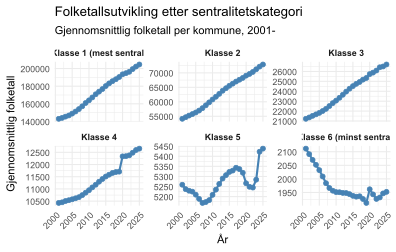
\includegraphics[keepaspectratio]{Arbeidskrav_Gruppe2_files/figure-pdf/unnamed-chunk-5-1.pdf}}

Folketallsutviklingen ser ut til å være lignende for de tre mest
sentrale sentralitetskategoriene. I klasse 4 ser vi en lignende, dog
svakere utvikling med et betraktelig hopp i folketall fra 2019 til 2020.
I klasse 5 var det befolkningsnedgang fra år 2000, før det snudde til
positiv utvikling rundt år 2007. Denne utviklingen snudde til det
negative igjen rundt 2016, før vi igjen ser et hopp i år 2020. De aller
minst sentrale kommunene har konsekvent hatt befolkningsnedgang siden
2000, foruten et hopp i 2020 og en mild oppgang de siste 2-3 årene.
Hoppet i 2020 skyldes kommunereformen. De minste kommunene (i folketall)
ble slått sammen for å spare på administrative utgifter, og det er
derfor vi ser størst hopp i folketall i de tre minst sentrale
kommunekategoriene i denne perioden. Den svake oppgangen i tiden etter
er interessant. Kan det være normalisering av hjemmekontor og økt fokus
på distriktsutvikling som driver denne desentraliseringen? \#\#\# Andel
innbyggere 20-29 år etter sentralitetskategori

\pandocbounded{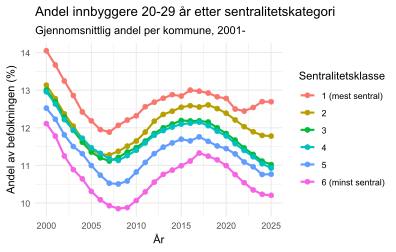
\includegraphics[keepaspectratio]{Arbeidskrav_Gruppe2_files/figure-pdf/unnamed-chunk-6-1.pdf}}

Andel innbyggere i 20-årene ser ut til å følge en noenlunde lik
utvikling nasjonalt, unntatt for sentralitetsklasse 1 og 2 som har hatt
en svakere nedgang i unge innbyggere enn resten av landet. Dette kan
stemme overens med antagelsen om at unge mennesker trekkes mot urbane
miljø.

\subsubsection{Arbeidsledighet etter
sentralitetskategori}\label{arbeidsledighet-etter-sentralitetskategori}

\pandocbounded{\includegraphics[keepaspectratio]{Arbeidskrav_Gruppe2_files/figure-pdf/unnamed-chunk-7-1.pdf}}

I figuren over ser vi en grafisk framstilling av gjennomsnittlig
arbeidsledighet (i prosent) i hver sentralitetskategori.
Arbeidsledigheten ser ut til å være relativt lik over hele landet, med
mindre enn ett prosentpoeng variasjon frem til 2020. I koronaåret 2020
ser vi en eksplosjon i ledighet for alle klassene, men med størst økning
i sentrale strøk. Sjokket fra COVID-19 ser ut til å ha gitt seg i 2022,
og grafen trender mot likevektsledighet igjen i 2023. Datagrunnlaget
viser at flere kommuner har oppgitt 0\% arbeidsledighet i 2024, og vi
antar at dette er en feil i statistikken.

\subsubsection{Sysselsettingsvekst etter
sentralitetskategori}\label{sysselsettingsvekst-etter-sentralitetskategori}

\pandocbounded{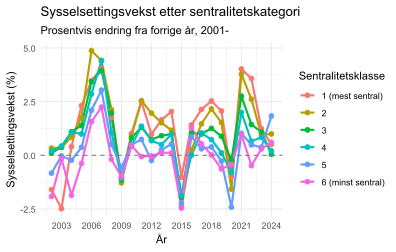
\includegraphics[keepaspectratio]{Arbeidskrav_Gruppe2_files/figure-pdf/unnamed-chunk-8-1.pdf}}

Figuren over viser sysselsettingsvekts. Vi ser positiv utvikling i de
fleste årene, unntatt negativ utvikling i 2009, 2015 og 2020. Dette kan
ses i forbindelse med internasjonale økonomiske trender. Nedgangen i
2009 kan forklares som en konsekvens av ``the great recession'' i 2008.
Nedgangen i 2015 kan vi forbinde med oljekrisen i 2014 da tusenvis av
nordmenn mistet jobbene sine i oljeindustrien som følge av et ras i
oljeprisen. Kyst-Norge er sterkt knyttet opp til oljeindustrien, og
ringvirkningene av dette oljeprisfallet kunne dermed føles sterkt også i
andre industrier i landet. Nedgangen i 2020 må ses i forbindelse med
koronapandemien.

\subsubsection{Kvadratmeterpris bolig}\label{kvadratmeterpris-bolig}

\pandocbounded{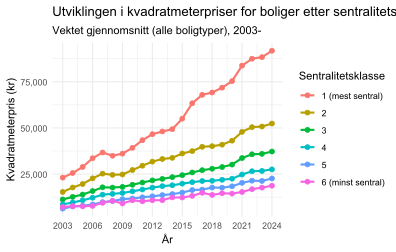
\includegraphics[keepaspectratio]{Arbeidskrav_Gruppe2_files/figure-pdf/unnamed-chunk-9-1.pdf}}

\pandocbounded{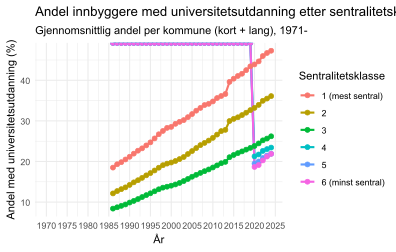
\includegraphics[keepaspectratio]{Arbeidskrav_Gruppe2_files/figure-pdf/unnamed-chunk-10-1.pdf}}

Kvadratmeterprisen på bolig har hatt en positiv utvikling over hele
landet, men den har vært aller sterkest i de mest sentrale kommunene.
Det er ellers interessant å se at kvadratmeterprisen ser ut til å
korreleres med sentralitet.

\subsubsection{Utvikling i utdanning}\label{utvikling-i-utdanning}

\pandocbounded{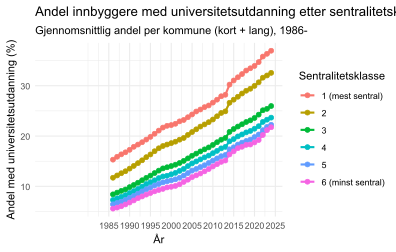
\includegraphics[keepaspectratio]{Arbeidskrav_Gruppe2_files/figure-pdf/unnamed-chunk-11-1.pdf}}

Utviklingen i andel høyt utdannede innbyggere har vært positiv
nasjonalt, men også her ser det ut til å korreleres med sentralitet. De
mest sentrale kommunene har også høyest andel høyt utdannede innbyggere.
Dette kan skyldes at befolkningen i bynære miljø har enklest tilgang til
universiteter og høyskoler, men det kan også være en indikasjon på at
det i bykommunene det er best tilgang på arbeid som krever høye
kvalifikasjoner. \#\#\# Utvikling i netto innflytting

\pandocbounded{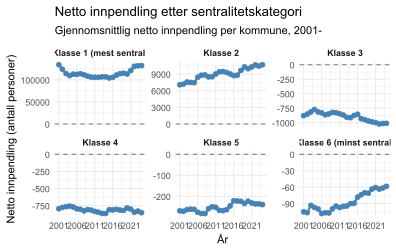
\includegraphics[keepaspectratio]{Arbeidskrav_Gruppe2_files/figure-pdf/unnamed-chunk-12-1.pdf}}

Grafene over må tydes med at negative tall viser positiv flyttebalanse
(altså mer innflytning enn utflytning).

\subsubsection{Utvikling i netto
innpendling}\label{utvikling-i-netto-innpendling}

\pandocbounded{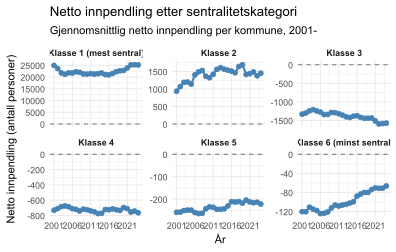
\includegraphics[keepaspectratio]{Arbeidskrav_Gruppe2_files/figure-pdf/unnamed-chunk-13-1.pdf}}

Grafene over viser netto innpendling etter sentralitetskategori. Vi ser
at for alle sentralitetsklassene utenom 1 og 2 har vi negativ
gjennomsnittsinnpendlig per kommune, altså vil det være flere arbeidere
som pendler ut fra kommunene enn pendler inn. Ett av målene for
sentralitetsindeksen er nemlig antall arbeidsplasser innenfor rimelig
pendleavstand (90 minutter) vektet etter nærhet. Det er dermed logisk at
det pendles mer inn til de mest sentrale kommunene.

\subsection{Korrelasjoner}\label{korrelasjoner}

\section{folketall vs andel\_20\_29(2013,
2023)}\label{folketall-vs-andel_20_292013-2023}

\begin{verbatim}
# A tibble: 2 x 2
     år   cor
  <int> <dbl>
1  2013 0.416
2  2023 0.386
\end{verbatim}

\section{sentralitet vs andel\_20\_29(2020,
2023)}\label{sentralitet-vs-andel_20_292020-2023}

\begin{verbatim}
# A tibble: 2 x 2
     år   cor
  <dbl> <dbl>
1  2020 0.261
2  2023 0.285
\end{verbatim}

\section{sentralitet vs arbeidsledighet(2020,
2023)}\label{sentralitet-vs-arbeidsledighet2020-2023}

\begin{verbatim}
# A tibble: 2 x 2
     år   cor
  <dbl> <dbl>
1  2020 0.470
2  2023 0.225
\end{verbatim}

\section{sentralitet vs bolig kvpris(Enebolig, 2020,
2023)}\label{sentralitet-vs-bolig-kvprisenebolig-2020-2023}

\begin{verbatim}
# A tibble: 2 x 2
     år   cor
  <dbl> <dbl>
1  2020 0.708
2  2023 0.715
\end{verbatim}

\section{sentralitet vs andel høyere utdanning(2020,
2023)}\label{sentralitet-vs-andel-huxf8yere-utdanning2020-2023}

\begin{verbatim}
# A tibble: 2 x 2
     år   cor
  <dbl> <dbl>
1  2020 0.587
2  2023 0.523
\end{verbatim}

\section{sentralitet vs utflytting per1000(2020,
2023)}\label{sentralitet-vs-utflytting-per10002020-2023}

\begin{verbatim}
# A tibble: 2 x 2
     år     cor
  <dbl>   <dbl>
1  2020  0.0802
2  2023 -0.0193
\end{verbatim}

\section{sentralitet vs innpend per1000(2020,
2023)}\label{sentralitet-vs-innpend-per10002020-2023}

\begin{verbatim}
# A tibble: 2 x 2
     år   cor
  <dbl> <dbl>
1  2020 0.371
2  2023 0.362
\end{verbatim}

\section{sentralitet vs utpend per1000(2020,
2023)}\label{sentralitet-vs-utpend-per10002020-2023}

\begin{verbatim}
# A tibble: 2 x 2
     år   cor
  <dbl> <dbl>
1  2020 0.606
2  2023 0.610
\end{verbatim}

\section{ledig vs andel\_20\_29(2013,
2023)}\label{ledig-vs-andel_20_292013-2023}

\begin{verbatim}
# A tibble: 2 x 2
     år    cor
  <int>  <dbl>
1  2013 0.0376
2  2023 0.0759
\end{verbatim}

\section{ledig vs bolig kvpris(Enebolig, 2013,
2023)}\label{ledig-vs-bolig-kvprisenebolig-2013-2023}

\begin{verbatim}
# A tibble: 2 x 2
     år    cor
  <int>  <dbl>
1  2013 -0.123
2  2023  0.169
\end{verbatim}

\section{ledig vs andel\_hoyere(2013,
2023)}\label{ledig-vs-andel_hoyere2013-2023}

\begin{verbatim}
# A tibble: 2 x 2
     år     cor
  <int>   <dbl>
1  2013 -0.102 
2  2023  0.0651
\end{verbatim}

\section{ledig vs flytt(brutto=utflytt, netto=nettoflytt)(2013,
2023)}\label{ledig-vs-flyttbruttoutflytt-nettonettoflytt2013-2023}

\begin{verbatim}
# A tibble: 2 x 3
     år cor_brutto cor_netto
  <int>      <dbl>     <dbl>
1  2013     0.137     0.0944
2  2023     0.0660   -0.0220
\end{verbatim}

\section{ledig vs pendl(brutto=utpend, netto=nettopend)(2013,
2023)}\label{ledig-vs-pendlbruttoutpend-nettonettopend2013-2023}

\begin{verbatim}
# A tibble: 2 x 3
     år cor_brutto cor_netto
  <int>      <dbl>     <dbl>
1  2013      0.143    0.0282
2  2023      0.228    0.0418
\end{verbatim}

\section{bolig kvpris vs andel\_hoyere(2013,
2023)}\label{bolig-kvpris-vs-andel_hoyere2013-2023}

\begin{verbatim}
# A tibble: 2 x 2
     år   cor
  <int> <dbl>
1  2013 0.759
2  2023 0.741
\end{verbatim}

\section{bolig kvpris vs andel\_20\_29(2013,
2023)}\label{bolig-kvpris-vs-andel_20_292013-2023}

\begin{verbatim}
# A tibble: 2 x 2
     år   cor
  <int> <dbl>
1  2013 0.832
2  2023 0.617
\end{verbatim}

\section{bolig kvpris vs innpend per1000(2013,
2023)}\label{bolig-kvpris-vs-innpend-per10002013-2023}

\begin{verbatim}
# A tibble: 2 x 2
     år   cor
  <int> <dbl>
1  2013 0.625
2  2023 0.701
\end{verbatim}

\section{bolig kvpris vs utpend per1000(2013,
2023)}\label{bolig-kvpris-vs-utpend-per10002013-2023}

\begin{verbatim}
# A tibble: 2 x 2
     år   cor
  <int> <dbl>
1  2013 0.724
2  2023 0.786
\end{verbatim}

\section{bolig kvpris vs utflytt per1000(2013,
2023)}\label{bolig-kvpris-vs-utflytt-per10002013-2023}

\begin{verbatim}
# A tibble: 2 x 2
     år     cor
  <int>   <dbl>
1  2013  0.372 
2  2023 -0.0286
\end{verbatim}

\section{bolig kvpris vs innflytt per1000(2013,
2023)}\label{bolig-kvpris-vs-innflytt-per10002013-2023}

\begin{verbatim}
# A tibble: 2 x 2
     år   cor
  <int> <dbl>
1  2013 0.704
2  2023 0.174
\end{verbatim}

\section{nettoflytt per1000 vs andel\_20\_29(2013,
2023)}\label{nettoflytt-per1000-vs-andel_20_292013-2023}

\begin{verbatim}
# A tibble: 2 x 2
     år     cor
  <int>   <dbl>
1  2013  0.0899
2  2023 -0.0588
\end{verbatim}

\section{nettoflytt per1000 vs netto utpend(= nettopend)(2013,
2023)}\label{nettoflytt-per1000-vs-netto-utpend-nettopend2013-2023}

\begin{verbatim}
# A tibble: 2 x 2
     år      cor
  <int>    <dbl>
1  2013  0.00251
2  2023 -0.00212
\end{verbatim}

\section{netto utpendling og bolig kvpris i tilgrensende
kommuner}\label{netto-utpendling-og-bolig-kvpris-i-tilgrensende-kommuner}

\begin{verbatim}
Spherical geometry (s2) switched off
\end{verbatim}

\begin{verbatim}
although coordinates are longitude/latitude, st_intersects assumes that they
are planar
\end{verbatim}

\begin{verbatim}
Warning in left_join(., kvpris_ene, by = c(nabo_knr = "kommunenummer")): Detected an unexpected many-to-many relationship between `x` and `y`.
i Row 1 of `x` matches multiple rows in `y`.
i Row 4130 of `y` matches multiple rows in `x`.
i If a many-to-many relationship is expected, set `relationship =
  "many-to-many"` to silence this warning.
\end{verbatim}

\begin{verbatim}
# A tibble: 2 x 2
     år    cor
  <int>  <dbl>
1  2013 -0.115
2  2023 -0.151
\end{verbatim}

\section{Paneldata, årlig endring i folketall og
sysselsetting}\label{paneldata-uxe5rlig-endring-i-folketall-og-sysselsetting}

\begin{verbatim}
# A tibble: 357 x 3
   kommunenummer n_obs cor_folk_syss
   <chr>         <int>         <dbl>
 1 0301             24       -0.0889
 2 1101             24        0.0797
 3 1103             24       -0.153 
 4 1106             24       -0.113 
 5 1108             24       -0.106 
 6 1111             24       -0.180 
 7 1112             24        0.0569
 8 1114             24       -0.197 
 9 1119             24        0.0467
10 1120             24        0.509 
# i 347 more rows
\end{verbatim}

\begin{verbatim}
# A tibble: 1 x 7
  n_komm   mean median    sd    min   max  n_na
   <int>  <dbl>  <dbl> <dbl>  <dbl> <dbl> <int>
1    357 0.0157 0.0153 0.226 -0.648 0.995     0
\end{verbatim}

\section{Paneldata, årlig endring i prosentvis arbeidsledighet og årlig
prosentvise endring i
sysselsetting}\label{paneldata-uxe5rlig-endring-i-prosentvis-arbeidsledighet-og-uxe5rlig-prosentvise-endring-i-sysselsetting}

\begin{verbatim}
# A tibble: 357 x 5
   kommunenummer n_obs sd_ledig sd_syss cor_ledig_syss
   <chr>         <int>    <dbl>   <dbl>          <dbl>
 1 0301             16    0.798    1.66        -0.855 
 2 1101             16    0.781    1.78        -0.506 
 3 1103             44    0.577    1.82        -0.837 
 4 1106             16    0.966    2.00        -0.734 
 5 1108             32    0.643    1.96        -0.398 
 6 1111             16    0.576    3.58         0.0591
 7 1112             16    0.487    3.47         0.289 
 8 1114             16    0.514    2.62        -0.297 
 9 1119             16    0.482    1.48        -0.263 
10 1120             16    0.742    2.27        -0.286 
# i 347 more rows
\end{verbatim}

\section{Paneldata, årlig endring i boligpriser og årlig netto
innflytting pr 1000
innbyggere}\label{paneldata-uxe5rlig-endring-i-boligpriser-og-uxe5rlig-netto-innflytting-pr-1000-innbyggere}

\begin{verbatim}
# A tibble: 192 x 5
   kommunenummer n_obs sd_kvpris sd_flytt cor_bolig_nettoflytt
   <chr>         <int>     <dbl>    <dbl>                <dbl>
 1 0301             14     2399.     1.25              -0.591 
 2 1101             14     1062.     1.73               0.157 
 3 1103             14     1568.     2.25              -0.408 
 4 1106             14      796.     1.31              -0.368 
 5 1108              4     1233.     2.00              -0.102 
 6 1111             14     1796.     3.03              -0.0138
 7 1112             11     1253.     4.12              -0.0224
 8 1114             11     2408.     4.05              -0.245 
 9 1119             14     1267.     2.98               0.0793
10 1120             14     1545.     1.91               0.208 
# i 182 more rows
\end{verbatim}

\section{Paneldata, årlig prosentvis endring i sysselsetting og årlig
endring i
boligpriser}\label{paneldata-uxe5rlig-prosentvis-endring-i-sysselsetting-og-uxe5rlig-endring-i-boligpriser}

\begin{verbatim}
# A tibble: 192 x 5
   kommunenummer n_obs sd_syss sd_kvpris cor_syss_bolig
   <chr>         <int>   <dbl>     <dbl>          <dbl>
 1 0301             22    1.86     2099.         0.379 
 2 1101             22    2.05     1143.         0.702 
 3 1103             22    3.38     1718.         0.601 
 4 1106             22    2.50      772.         0.583 
 5 1108              4    1.45     1233.         0.576 
 6 1111             20    4.63     1614.         0.0927
 7 1112             15    3.97     1331.         0.177 
 8 1114             14    3.13     2224.         0.172 
 9 1119             22    1.89     1184.         0.272 
10 1120             22    2.24     1516.         0.512 
# i 182 more rows
\end{verbatim}

\section{Paneldata, årlige endring i innpendling pr 1000 innbyggere og
årlig prosentvis endring i
sysselsetting}\label{paneldata-uxe5rlige-endring-i-innpendling-pr-1000-innbyggere-og-uxe5rlig-prosentvis-endring-i-sysselsetting}

\begin{verbatim}
# A tibble: 357 x 5
   kommunenummer n_obs sd_innpend sd_syss cor_innpend_syss
   <chr>         <int>      <dbl>   <dbl>            <dbl>
 1 0301             24     4900.     2.03            0.933
 2 1101             24       61.0    2.02            0.808
 3 1103             24     1826.     3.36            0.948
 4 1106             24      301.     2.41            0.948
 5 1108             24      752.     2.84            0.955
 6 1111             24       36.6    3.78            0.844
 7 1112             24       31.2    3.99            0.894
 8 1114             24       20.1    2.59            0.736
 9 1119             24       66.1    2.06            0.826
10 1120             24      127.     2.51            0.900
# i 347 more rows
\end{verbatim}

\subsection{Lagge en variabel}\label{lagge-en-variabel}

For enkelte relasjoner, som mellom boligpriser og flytting, er det
rimelig å anta at virkninger oppstår med tidsforsinkelse. Vi lagger
derfor boligprisene ett år for å ta hensyn til tregheter i
husholdningenes tilpasning.

\subsubsection{Demeaning}\label{demeaning}

\begin{verbatim}
# A tibble: 1 x 1
      cor
    <dbl>
1 -0.0290
\end{verbatim}

Demeaning fjerner tidsinvariante kommuneegenskaper som geografisk
beliggenhet, størrelse og historisk sentralitet. Dette gjør at
korrelasjonene i større grad reflekterer samvariasjon over tid innen
samme kommune, snarere enn strukturelle forskjeller mellom kommuner.
Dette er særlig nyttig i paneldata, der en kan risikere uekte
korrelasjoner som er drevet av permanente nivåforskjeller.

\subsection{Pearson vs Spearman}\label{pearson-vs-spearman}

Beregner en Spearman korrelasjonskoeffisient og en Pearson
korrelasjonskoeffsient. Spearman-korrelasjon måler styrken og retningen
til variablene som beveger seg i samme retning, uavhengig av om
sammenhengen er lineær, mens Pearson-korrelasjon målers den lineære
styrken og retningen til variablene mens de beveger seg kontinuerlig. Vi
tar eksempelet mellom sentralitet og kvadratmeterpris

\begin{verbatim}
# A tibble: 1 x 2
  pearson spearman
    <dbl>    <dbl>
1   0.715    0.710
\end{verbatim}

Pearson- og Spearman-korrelasjonene er svært like i størrelse (0,715 og
0,710). Dette indikerer at sammenhengen mellom variablene er tilnærmet
lineær, og at resultatet ikke i vesentlig grad påvirkes av uteliggere
eller skjev fordeling. Rangeringen av kommunene samsvarer godt med
nivåforskjellene i variablene, noe som tyder på en stabil og systematisk
samvariasjon.

\subsection{Velg ut noen sammenhenger for visualisering med
spredningsdiagrammer}\label{velg-ut-noen-sammenhenger-for-visualisering-med-spredningsdiagrammer}

\begin{verbatim}
`geom_smooth()` using formula = 'y ~ x'
\end{verbatim}

\begin{verbatim}
Warning: Removed 88 rows containing non-finite outside the scale range
(`stat_smooth()`).
\end{verbatim}

\begin{verbatim}
Warning: Removed 88 rows containing missing values or values outside the scale range
(`geom_point()`).
\end{verbatim}

\pandocbounded{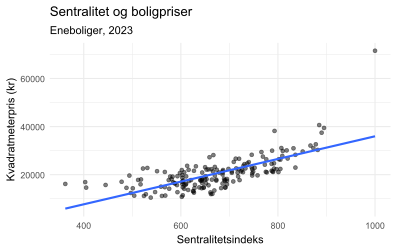
\includegraphics[keepaspectratio]{Arbeidskrav_Gruppe2_files/figure-pdf/unnamed-chunk-48-1.pdf}}

Spredningsdiagrammet viser en klart stigende og tilnærmet lineær
sammenheng, noe som støtter bruk av Pearson-korrelasjon.

\begin{verbatim}
`geom_smooth()` using formula = 'y ~ x'
\end{verbatim}

\pandocbounded{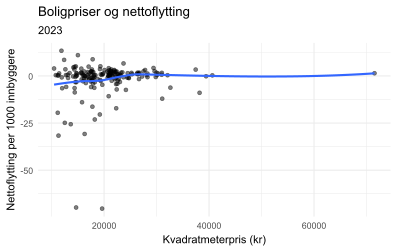
\includegraphics[keepaspectratio]{Arbeidskrav_Gruppe2_files/figure-pdf/unnamed-chunk-49-1.pdf}}

Figuren indikerer en monoton, men ikke-lineær sammenheng, med betydelig
spredning. Dette tilsier at Spearman-korrelasjonen gir et mer robust mål
enn Pearson

Korrelasjonskoeffisientene gir kun informasjon om samvariasjon, som er
et statistiks mål på strken og retningen, men kan ikke helt tolke
årsaksbestemmelsen. Sammenhengene kan være påvirket av simultanitet,
utelatte variabler og strukturelle forskjeller mellom kommuner. Videre
kan aggregert kommunedata skjule betydelig intern ulikheter. Resultatene
bør derfor tolkes som deskriptive, og primært brukes som grunnlag for
videre analyse.

\subsection{Systematiske forskjeller mellom kommuner i ulike
sentralitetskategorier}\label{systematiske-forskjeller-mellom-kommuner-i-ulike-sentralitetskategorier}

\begin{verbatim}
# A tibble: 6 x 3
  `Klasse 2023`     cor     n
          <dbl>   <dbl> <int>
1             1 -0.418     19
2             2  0.135     67
3             3 -0.0697   234
4             4  0.128    436
5             5  0.136    596
6             6  0.0861   214
\end{verbatim}

Korrelasjonsanalysene viser at sammenhengen varierer systematisk mellom
kommuner i ulike sentralitetskategorier. For de fleste
sentralitetsklasser (2--6) er korrelasjonen mellom variablene svak og
svakt positiv. I de mest sentrale kommunene (klasse 1) er sammenhengen
derimot klart negativ. Dette kan indikere at svært høye boligpriser i de
største bykommunene bidrar til å begrense netto innflytting, blant annet
ved at flere husholdninger velger å bosette seg i omlandskommuner og
pendle inn til byene. Samtidig er antall observasjoner i denne gruppen
lavt, noe som tilsier at resultatene bør tolkes med forsiktighet.
Korrelasjonen mellom boligpriser og nettoflytting er sterkere i store
byer enn i distriktskommuner, noe som kan indikere at boligmarkedet
spiller en mer aktiv rolle i flyttebeslutninger i urbane strøk. Videre
kan en forvente at sammenhengene varierer systematisk mellom ulike typer
kommuner, slik de er klassifisert hos Andersson et al.~(2020). For
eksempel kan relasjonen mellom sysselsetting, boligpriser og flytting
være sterkere i funksjonelle byregioner enn i perifere
distriktskommuner. Dette gir derimot ikke et helt grunnlag for kausale
tolkninger men kan indikere systematiske samvariasjoner som danner
utgangspunkt for videre analyser og hypoteser.

\subsection{Forskjeller mellom kommuner i ulike kategorier hos Andersson
et
al.~(2020)}\label{forskjeller-mellom-kommuner-i-ulike-kategorier-hos-andersson-et-al.-2020}

\begin{verbatim}
# A tibble: 4 x 3
  andersson_type         cor     n
  <chr>                <dbl> <int>
1 Forstad / omland     0.135    67
2 Perifere distrikter  0.117   810
3 Regionale sentra     0.164   670
4 Storbykjerne        -0.418    19
\end{verbatim}

Analysene viser tydelige forskjeller mellom kommuner gruppert etter en
forenklet typologi inspirert av Andersson et al.~(2020). For
storbykjerner er korrelasjonen mellom boligpriser og nettoflytting klart
negativ, noe som indikerer at svært høye boligpriser i de største
bykommunene kan virke begrensende på netto innflytting. For regionale
sentra, forstads- og omlandskommuner samt perifere distriktskommuner er
sammenhengen derimot svakt positiv. Dette kan tolkes som at boligpriser
i disse områdene i større grad reflekterer attraktivitet og
etterspørsel, uten de samme kapasitetsbegrensningene som i
storbykjerner. Her er også antall observasjoner for storbykjerner
relativt lavt, noe som tilsier at resultatene bør tolkes med en viss
varsomhet. Resultatene understøtter dermed antakelsen om at sammenhenger
mellom boligmarked og flytteprosesser varierer systematisk med
kommunenes funksjonelle rolle i det regionale systemet.

\section{4.Sammenhengen mellom befolkning og
sysselsetting}\label{sammenhengen-mellom-befolkning-og-sysselsetting}

\begin{table}
\centering
\begin{talltblr}[         %% tabularray outer open
entry=none,label=none,
note{}={+ p \num{< 0.1}, * p \num{< 0.05}, ** p \num{< 0.01}, *** p \num{< 0.001}},
]                     %% tabularray outer close
{                     %% tabularray inner open
colspec={Q[]Q[]Q[]},
column{2-3}={}{halign=c,},
column{1}={}{halign=l,},
hline{6}={1-3}{solid, black, 0.05em},
}                     %% tabularray inner close
\toprule
& Pooled OLS & Kommune + år FE \\ \midrule %% TinyTableHeader
(Intercept) & \num{-2254.159}*** &  \\
& (\num{47.010}) &  \\
befolkning & \num{0.676}*** & \num{0.589}*** \\
& (\num{0.001}) & (\num{0.021}) \\
Num.Obs. & \num{8925} & \num{8925} \\
R2 & \num{0.976} & \num{0.999} \\
R2 Within &  & \num{0.871} \\
Std.Errors &  & by: kommunenummer \\
\bottomrule
\end{talltblr}
\end{table}

Sammenlign resultatene for disse to regresjonsmodellene:

I den pooled regresjonen er sysselsetting den avhengige variabelen og
befolkning forklaringsvariabelen. Modellen skiller ikke mellom kommuner
og år, men behandler alle kommune-år-observasjoner samlet. Estimatet
utnytter derfor både forskjeller mellom kommuner og endringer innen
samme kommune over tid for å beskrive sammenhengen mellom befolkning og
sysselsetting. Koeffisienten på 0,696 innebærer at en økning i
befolkningen på en person i gjennomsnitt er assosiert med om lag 0,696
flere sysselsatte.

Når faste effekter for både kommuner og år inkluderes, kontrollerer
modellen for kommune-spesifikke faktorer som er konstante over tid, samt
felles nasjonale sjokk i hvert år. I denne spesifikasjonen identifiseres
sammenhengen mellom befolkning og sysselsetting utelukkende ved hjelp av
variasjon innen samme kommune over tid. Koeffisienten på 0,601 innebærer
at en økning i befolkningen på en person innen en kommune i gjennomsnitt
er assosiert med om lag 0,601 flere sysselsatte.

At koeffisienten i modellen med faste effekter er lavere enn i den
pooled regresjonen, indikerer at en del av den positive sammenhengen i
pooled modellen skyldes varige strukturelle forskjeller mellom kommuner
som kontrolleres for når faste effekter inkluderes.

Sammenlign med resultater for korrelasjonskoeffisienter i deloppgaven
foran:

Kan resultatene fra slike regresjonsmodeller i større grad enn
korrelasjonskoeffisienten tolkes kausalt?

Resultatene fra regresjonsmodellene kan i større grad enn en enkel
korrelasjonskoeffisient tolkes kausalt. En korrelasjonskoeffisient viser
kun om to variabler samvarierer. Den kontrollerer ikke for andre
forhold. Regresjonsmodellene kontrollerer derimot for flere viktige
faktorer. Når faste effekter for kommuner og år inkluderes, tas det
hensyn til både varige forskjeller mellom kommuner og felles sjokk som
rammer alle kommuner i samme år. Estimatene bygger da på endringer innen
samme kommune over tid. Dette gir et bedre grunnlag for kausal tolkning.
Likevel kan resultatene ikke tolkes som fullt ut kausale. Det kan
fortsatt finnes omvendt kausalitet og tidsvarierende forhold som ikke er
kontrollert for i modellen.

\section{6. En multippel regresjonsmodell for
folketallsutvikling}\label{en-multippel-regresjonsmodell-for-folketallsutvikling}

\subsubsection{start-år-modell}\label{start-uxe5r-modell}

\begin{verbatim}

Call:
lm(formula = folketallsvekst ~ sentralitet + arbeidsledighet_pct + 
    hoyere_utdanning_andel + sysselsetting_per1000 + netto_innpendling_per1000 + 
    netto_utflytting_per1000 + ln_boligpris + andel_20_29 + factor(landsdel), 
    data = df_6_csA)

Residuals:
     Min       1Q   Median       3Q      Max 
-12.2214  -1.9365  -0.4556   1.3411  18.4082 

Coefficients:
                              Estimate   Std. Error t value
(Intercept)               -22.68322610   7.36548663  -3.080
sentralitet                 0.01872326   0.00276729   6.766
arbeidsledighet_pct        -0.73477563   0.25566456  -2.874
hoyere_utdanning_andel     -0.29479627   0.04790442  -6.154
sysselsetting_per1000      -0.00001328   0.00207137  -0.006
netto_innpendling_per1000   0.00013866   0.00003324   4.172
netto_utflytting_per1000   -0.14800636   0.03524131  -4.200
ln_boligpris                1.02422914   0.89035638   1.150
andel_20_29                67.82872472  12.04418432   5.632
factor(landsdel)sør         1.99289961   0.50692117   3.931
factor(landsdel)vest        4.11452354   0.47631365   8.638
factor(landsdel)Trøndelag   2.25121239   0.59629797   3.775
factor(landsdel)nord        2.51294555   0.63766844   3.941
                                      Pr(>|t|)    
(Intercept)                           0.002181 ** 
sentralitet                    0.0000000000357 ***
arbeidsledighet_pct                   0.004219 ** 
hoyere_utdanning_andel         0.0000000015077 ***
sysselsetting_per1000                 0.994888    
netto_innpendling_per1000      0.0000353855993 ***
netto_utflytting_per1000       0.0000314140496 ***
ln_boligpris                          0.250523    
andel_20_29                    0.0000000291983 ***
factor(landsdel)sør            0.0000958466449 ***
factor(landsdel)vest      < 0.0000000000000002 ***
factor(landsdel)Trøndelag             0.000178 ***
factor(landsdel)nord           0.0000922512419 ***
---
Signif. codes:  0 '***' 0.001 '**' 0.01 '*' 0.05 '.' 0.1 ' ' 1

Residual standard error: 3.684 on 522 degrees of freedom
Multiple R-squared:  0.3935,    Adjusted R-squared:  0.3796 
F-statistic: 28.22 on 12 and 522 DF,  p-value: < 0.00000000000000022
\end{verbatim}

\subsubsection{periode-gjennomsnitt-modell}\label{periode-gjennomsnitt-modell}

\begin{verbatim}

Call:
lm(formula = folketallsvekst ~ sentralitet + arbeidsledighet_pct + 
    hoyere_utdanning_andel + sysselsetting_per1000 + netto_innpendling_per1000 + 
    netto_utflytting_per1000 + ln_boligpris + andel_20_29 + landsdel, 
    data = df_6_csB)

Residuals:
     Min       1Q   Median       3Q      Max 
-12.6748  -2.6629  -0.6332   1.9477  17.7698 

Coefficients:
                              Estimate   Std. Error t value        Pr(>|t|)    
(Intercept)               -41.05309693  13.87074272  -2.960        0.003351 ** 
sentralitet                 0.01783805   0.00518823   3.438        0.000677 ***
arbeidsledighet_pct        -0.43702274   0.61251725  -0.713        0.476157    
hoyere_utdanning_andel     -0.31960682   0.08524760  -3.749        0.000217 ***
sysselsetting_per1000      -0.00112992   0.00345739  -0.327        0.744061    
netto_innpendling_per1000   0.00013067   0.00004161   3.140        0.001873 ** 
netto_utflytting_per1000   -0.11551935   0.05912694  -1.954        0.051755 .  
ln_boligpris                2.76513828   1.67533458   1.650        0.099995 .  
andel_20_29                87.42684340  22.75080892   3.843        0.000151 ***
landsdelsør                 2.13636058   0.90642567   2.357        0.019137 *  
landsdelvest                5.60620310   0.81542857   6.875 0.0000000000423 ***
landsdelTrøndelag           3.18265930   1.07132375   2.971        0.003236 ** 
landsdelnord                2.94233937   1.11890264   2.630        0.009034 ** 
---
Signif. codes:  0 '***' 0.001 '**' 0.01 '*' 0.05 '.' 0.1 ' ' 1

Residual standard error: 4.574 on 272 degrees of freedom
Multiple R-squared:  0.3922,    Adjusted R-squared:  0.3654 
F-statistic: 14.63 on 12 and 272 DF,  p-value: < 0.00000000000000022
\end{verbatim}

\subsubsection{FE-modell}\label{fe-modell}

\begin{verbatim}
NOTE: 2/0 fixed-effect singletons were removed (2 observations).
\end{verbatim}

\begin{verbatim}
Warning: The VCOV matrix is not positive semi-definite and was 'fixed' (see
?vcov).
\end{verbatim}

\begin{verbatim}
OLS estimation, Dep. Var.: dlog_folketall
Observations: 1,964
Fixed-effects: kommunenummer: 282,  år: 15
Standard-errors: Clustered (kommunenummer) 
                              Estimate Std. Error   t value  Pr(>|t|)    
arbeidsledighet_pct        0.000402380 0.00054810  0.734139 0.4634764    
hoyere_utdanning_andel     0.000495563 0.00077970  0.635579 0.5255680    
sysselsetting_per1000      0.000032864 0.00002220  1.480209 0.1399376    
netto_innpendling_per1000 -0.000000544 0.00000101 -0.541228 0.5887796    
netto_utflytting_per1000   0.000566743 0.00006454  8.781164 < 2.2e-16 ***
ln_boligpris               0.001265786 0.00324323  0.390286 0.6966210    
andel_20_29                0.194743092 0.06506961  2.992843 0.0030095 ** 
---
Signif. codes:  0 '***' 0.001 '**' 0.01 '*' 0.05 '.' 0.1 ' ' 1
RMSE: 0.00779     Adj. R2: 0.408679
                Within R2: 0.096905
\end{verbatim}

\section{7. En multippel regresjonsmodell for
sysselsettingsvekst}\label{en-multippel-regresjonsmodell-for-sysselsettingsvekst}

\subsubsection{start-år-modell}\label{start-uxe5r-modell-1}

\begin{verbatim}

Call:
lm(formula = sysselsettingsvekst ~ folketallsvekst + sentralitet + 
    arbeidsledighet_pct + hoyere_utdanning_andel + sysselsetting_per1000 + 
    netto_innpendling_per1000 + netto_utflytting_per1000 + ln_boligpris + 
    andel_20_29 + factor(landsdel), data = df_7_csA)

Residuals:
    Min      1Q  Median      3Q     Max 
-27.490  -2.475  -0.176   2.436  31.834 

Coefficients:
                               Estimate    Std. Error t value
(Intercept)               -51.016618639  16.113013991  -3.166
folketallsvekst             0.926928130   0.088780841  10.441
sentralitet                -0.016309904   0.005919227  -2.755
arbeidsledighet_pct         1.514245924   0.545816970   2.774
hoyere_utdanning_andel      0.116715463   0.112903140   1.034
sysselsetting_per1000       0.000825499   0.004599957   0.179
netto_innpendling_per1000   0.000001053   0.000062296   0.017
netto_utflytting_per1000   -0.198829842   0.129980618  -1.530
ln_boligpris                5.868627959   1.953153641   3.005
andel_20_29                 8.183514948  31.419159634   0.260
factor(landsdel)sør        -0.662665315   1.240768283  -0.534
factor(landsdel)vest       -0.903816654   1.008854458  -0.896
factor(landsdel)Trøndelag  -1.454352411   1.172113935  -1.241
factor(landsdel)nord        1.807183376   1.421858749   1.271
                                      Pr(>|t|)    
(Intercept)                            0.00168 ** 
folketallsvekst           < 0.0000000000000002 ***
sentralitet                            0.00617 ** 
arbeidsledighet_pct                    0.00584 ** 
hoyere_utdanning_andel                 0.30197    
sysselsetting_per1000                  0.85768    
netto_innpendling_per1000              0.98652    
netto_utflytting_per1000               0.12702    
ln_boligpris                           0.00285 ** 
andel_20_29                            0.79466    
factor(landsdel)sør                    0.59363    
factor(landsdel)vest                   0.37094    
factor(landsdel)Trøndelag              0.21553    
factor(landsdel)nord                   0.20459    
---
Signif. codes:  0 '***' 0.001 '**' 0.01 '*' 0.05 '.' 0.1 ' ' 1

Residual standard error: 6.275 on 343 degrees of freedom
Multiple R-squared:  0.4289,    Adjusted R-squared:  0.4073 
F-statistic: 19.81 on 13 and 343 DF,  p-value: < 0.00000000000000022
\end{verbatim}

\subsubsection{periode-gjennomsnitt-modell}\label{periode-gjennomsnitt-modell-1}

\begin{verbatim}

Call:
lm(formula = sysselsettingsvekst ~ folketallsvekst + sentralitet + 
    arbeidsledighet_pct + hoyere_utdanning_andel + sysselsetting_per1000 + 
    netto_innpendling_per1000 + netto_utflytting_per1000 + ln_boligpris + 
    andel_20_29 + factor(landsdel), data = df_7_csB)

Residuals:
     Min       1Q   Median       3Q      Max 
-25.8024  -3.3918  -0.1199   3.0578  27.0748 

Coefficients:
                              Estimate   Std. Error t value         Pr(>|t|)
(Intercept)               -59.30601250  29.97423135  -1.979          0.04938
folketallsvekst             0.85377007   0.11185631   7.633 0.00000000000127
sentralitet                -0.01506838   0.01007074  -1.496          0.13633
arbeidsledighet_pct         1.44469902   1.23041606   1.174          0.24188
hoyere_utdanning_andel      0.06406474   0.19007930   0.337          0.73648
sysselsetting_per1000       0.01863085   0.00702242   2.653          0.00869
netto_innpendling_per1000  -0.00003746   0.00007407  -0.506          0.61366
netto_utflytting_per1000   -0.38273385   0.17412183  -2.198          0.02921
ln_boligpris                6.41049561   3.59944387   1.781          0.07659
andel_20_29               -24.33424496  54.74012449  -0.445          0.65718
factor(landsdel)sør         0.20632221   2.12435502   0.097          0.92274
factor(landsdel)vest       -1.47916336   1.63936488  -0.902          0.36811
factor(landsdel)Trøndelag  -2.46159915   1.94698271  -1.264          0.20774
factor(landsdel)nord       -0.04767269   2.24631505  -0.021          0.98309
                             
(Intercept)               *  
folketallsvekst           ***
sentralitet                  
arbeidsledighet_pct          
hoyere_utdanning_andel       
sysselsetting_per1000     ** 
netto_innpendling_per1000    
netto_utflytting_per1000  *  
ln_boligpris              .  
andel_20_29                  
factor(landsdel)sør          
factor(landsdel)vest         
factor(landsdel)Trøndelag    
factor(landsdel)nord         
---
Signif. codes:  0 '***' 0.001 '**' 0.01 '*' 0.05 '.' 0.1 ' ' 1

Residual standard error: 7.409 on 181 degrees of freedom
Multiple R-squared:  0.4573,    Adjusted R-squared:  0.4183 
F-statistic: 11.73 on 13 and 181 DF,  p-value: < 0.00000000000000022
\end{verbatim}

\subsubsection{FE-modell}\label{fe-modell-1}

\begin{verbatim}
NOTE: 2/0 fixed-effect singletons were removed (2 observations).
\end{verbatim}

\begin{verbatim}
Warning: The VCOV matrix is not positive semi-definite and was 'fixed' (see
?vcov).
\end{verbatim}

\begin{verbatim}
OLS estimation, Dep. Var.: dlog_sysselsetting
Observations: 1,964
Fixed-effects: kommunenummer: 282,  år: 15
Standard-errors: Clustered (kommunenummer) 
                             Estimate Std. Error   t value         Pr(>|t|)    
dlog_folketall             0.32531359 0.08528247  3.814542 0.00016777681060 ***
arbeidsledighet_pct       -0.00977435 0.00234186 -4.173763 0.00003999230587 ***
hoyere_utdanning_andel     0.00184426 0.00198452  0.929324 0.35351893460208    
sysselsetting_per1000      0.00056485 0.00008769  6.441608 0.00000000051111 ***
netto_innpendling_per1000 -0.00000146 0.00000102 -1.425005 0.15526554201819    
netto_utflytting_per1000   0.00031320 0.00016747  1.870189 0.06249716244416 .  
ln_boligpris              -0.02098985 0.00946443 -2.217760 0.02737100025999 *  
andel_20_29               -0.44528050 0.17564886 -2.535061 0.01178540012032 *  
---
Signif. codes:  0 '***' 0.001 '**' 0.01 '*' 0.05 '.' 0.1 ' ' 1
RMSE: 0.020758     Adj. R2: 0.241932
                 Within R2: 0.185363
\end{verbatim}

\section{Litteraturliste}\label{litteraturliste}

\phantomsection\label{refs}
\begin{CSLReferences}{1}{0}
\bibitem[\citeproctext]{ref-modelsummary2022}
Arel-Bundock, V. (2022). {modelsummary}: Data and model summaries in
{R}. \emph{Journal of Statistical Software}, \emph{103}(1), 1--23.
\url{https://doi.org/10.18637/jss.v103.i01}

\bibitem[\citeproctext]{ref-R-modelsummary}
Arel-Bundock, V. (2025). \emph{Modelsummary: Summary tables and plots
for statistical models and data: Beautiful, customizable, and
publication-ready}. \url{https://modelsummary.com}

\bibitem[\citeproctext]{ref-R-spdep}
Bivand, R. (2025). \emph{Spdep: Spatial dependence: Weighting schemes,
statistics}. \url{https://github.com/r-spatial/spdep/}

\bibitem[\citeproctext]{ref-spdep2013}
Bivand, R. S., Pebesma, E., \& Gómez-Rubio, V. (2013). \emph{Applied
spatial data analysis with {R}, second edition}. Springer, NY.
\url{https://asdar-book.org/}

\bibitem[\citeproctext]{ref-spdep2018}
Bivand, R., \& Wong, D. W. S. (2018). Comparing implementations of
global and local indicators of spatial association. \emph{TEST},
\emph{27}(3), 716--748. \url{https://doi.org/10.1007/s11749-018-0599-x}

\bibitem[\citeproctext]{ref-R-flextable}
Gohel, D., \& Skintzos, P. (2025). \emph{Flextable: Functions for
tabular reporting}. \url{https://ardata-fr.github.io/flextable-book/}

\bibitem[\citeproctext]{ref-lubridate2011}
Grolemund, G., \& Wickham, H. (2011). Dates and times made easy with
{lubridate}. \emph{Journal of Statistical Software}, \emph{40}(3),
1--25. \url{https://www.jstatsoft.org/v40/i03/}

\bibitem[\citeproctext]{ref-erikherstadhorgen2025}
Horgen, E. H. (2025). Hvorfor ulike arbeidsledighetstall? In \emph{SSB}.
\url{https://www.ssb.no/arbeid-og-lonn/sysselsetting/artikler/hvorfor-ulike-arbeidsledighetstall}

\bibitem[\citeproctext]{ref-huxf8ydahl}
Høydahl, E. (n.d.). \emph{Sentralitetsindeksen. Oppdatering med
2020-kommuner}.

\bibitem[\citeproctext]{ref-hvorfor2025}
Hvorfor ulike arbeidsledighetstall? (2025). In \emph{SSB}.
\url{https://www.ssb.no/arbeid-og-lonn/sysselsetting/artikler/hvorfor-ulike-arbeidsledighetstall}

\bibitem[\citeproctext]{ref-R-PxWebApiData}
Langsrud, Ø., \& Bruusgaard, J. (2024). \emph{PxWebApiData: PX-web data
by API}. \url{https://statisticsnorway.github.io/ssb-pxwebapidata/}

\bibitem[\citeproctext]{ref-R-writexl}
Ooms, J. (2025). \emph{Writexl: Export data frames to excel xlsx
format}. \url{https://ropensci.r-universe.dev/writexl}

\bibitem[\citeproctext]{ref-sf2018}
Pebesma, E. (2018). {Simple Features for R: Standardized Support for
Spatial Vector Data}. \emph{{The R Journal}}, \emph{10}(1), 439--446.
\url{https://doi.org/10.32614/RJ-2018-009}

\bibitem[\citeproctext]{ref-R-sf}
Pebesma, E. (2025). \emph{Sf: Simple features for r}.
\url{https://r-spatial.github.io/sf/}

\bibitem[\citeproctext]{ref-sf2023}
Pebesma, E., \& Bivand, R. (2023a). \emph{{Spatial Data Science: With
applications in R}}. {Chapman and Hall/CRC}.
\url{https://doi.org/10.1201/9780429459016}

\bibitem[\citeproctext]{ref-spdep2023}
Pebesma, E., \& Bivand, R. S. (2023b). \emph{Spatial data science with
applications in {R}}. Chapman \& Hall. \url{https://r-spatial.org/book/}

\bibitem[\citeproctext]{ref-spdep2022}
Roger Bivand. (2022). R packages for analyzing spatial data: A
comparative case study with areal data. \emph{Geographical Analysis},
\emph{54}(3), 488--518. \url{https://doi.org/10.1111/gean.12319}

\bibitem[\citeproctext]{ref-statistisksentralbyruxe52025}
Sentralbyrå, S. (2025). Hvorfor ulike arbeidsledighetstall? In
\emph{SSB}.
\url{https://www.ssb.no/arbeid-og-lonn/sysselsetting/artikler/hvorfor-ulike-arbeidsledighetstall}

\bibitem[\citeproctext]{ref-R-lubridate}
Spinu, V., Grolemund, G., \& Wickham, H. (2024). \emph{Lubridate: Make
dealing with dates a little easier}.
\url{https://lubridate.tidyverse.org}

\bibitem[\citeproctext]{ref-spuxf8rsmuxe5l2025}
\emph{Spørsmål og svar om arbeidsledighet i norge}. (2025).
\url{https://arbeidsledighet.no/sporsmal-og-svar/}

\bibitem[\citeproctext]{ref-R-tidyverse}
Wickham, H. (2023). \emph{Tidyverse: Easily install and load the
tidyverse}. \url{https://tidyverse.tidyverse.org}

\bibitem[\citeproctext]{ref-tidyverse2019}
Wickham, H., Averick, M., Bryan, J., Chang, W., McGowan, L. D.,
François, R., Grolemund, G., Hayes, A., Henry, L., Hester, J., Kuhn, M.,
Pedersen, T. L., Miller, E., Bache, S. M., Müller, K., Ooms, J.,
Robinson, D., Seidel, D. P., Spinu, V., \ldots{} Yutani, H. (2019).
Welcome to the {tidyverse}. \emph{Journal of Open Source Software},
\emph{4}(43), 1686. \url{https://doi.org/10.21105/joss.01686}

\bibitem[\citeproctext]{ref-R-readxl}
Wickham, H., \& Bryan, J. (2025). \emph{Readxl: Read excel files}.
\url{https://readxl.tidyverse.org}

\bibitem[\citeproctext]{ref-R-dplyr}
Wickham, H., François, R., Henry, L., Müller, K., \& Vaughan, D. (2023).
\emph{Dplyr: A grammar of data manipulation}.
\url{https://dplyr.tidyverse.org}

\bibitem[\citeproctext]{ref-knitr2014}
Xie, Y. (2014). Knitr: A comprehensive tool for reproducible research in
{R}. In V. Stodden, F. Leisch, \& R. D. Peng (Eds.), \emph{Implementing
reproducible computational research}. Chapman; Hall/CRC.

\bibitem[\citeproctext]{ref-knitr2015}
Xie, Y. (2015). \emph{Dynamic documents with {R} and knitr} (2nd ed.).
Chapman; Hall/CRC. \url{https://yihui.org/knitr/}

\bibitem[\citeproctext]{ref-R-knitr}
Xie, Y. (2025). \emph{Knitr: A general-purpose package for dynamic
report generation in r}. \url{https://yihui.org/knitr/}

\end{CSLReferences}

\listoffigures
\listoftables




\end{document}
